\chapter{Converse and Model Analysis}

\section{The Computational Problem Solving Cycle\label{sec:computational_problem_cycle}}

Business analytics is about using data and models  to solve---or at least to contribute towards solving---decision problems faced by individuals and organizations of all sorts. These include commercial and non-profit ventures, LLCs, privately-held firms, ESOPs, cooperatives, governmental organizations, NGOs, and even quangos. Business analytics is, above all, about ``thinking with models and data'' (including text data); it is about using them as inputs to  deliberative processes that typically are embedded in a rich context of application, which itself also provides inputs to the decision maker.  

Focusing on the general analytics at the expense of details of the governing context of any particular case, there are three kinds of knowledge important for our subject.

\begin{enumerate}
\item Encoding.

How to express an algorithm or procedure in the computational environment of our choice and get it to run and produce useful results?

Important modern computational environments include Excel (and other spreadsheet programs), \mlb , Mathematica, Python, Ruby, PHP, JavaScript, R, SAS, SPSS, NetLogo, and much else, including core programming languages such as C, C++, and Java.

We shall discuss coding in this book, but for the most part relegate it to later chapters, aimed at more advanced users, or at least users who would be more advanced and so wish to study programming for business analytics. Python and NetLogo will serve as our focal core programming languages, although we shall have many occasions to mention others. We will advert to Excel, GAMS, and OPL often, focusing on NetLogo and Excel in the early parts of the book.

%\begin{enumerate}
%\item General programming constructs in the language, e.g., variables, control flow, I/O, etc.
%\item Language-specific features, e.g., arrays and operations on them in \mlb , Toolboxes, etc.
%\end{enumerate}

\item Solution design.

Solution design is an issue that arises prior to encoding. Given a problem, how should it be represented so that  it  can be coded in one's computational environment of choice (NetLogo, Python, Excel, etc.)? Alternatively put:
 How should we  design the representations---the data structures and algorithms---for solving the problem?
 
 Solution design, including representation, efforts occur at a level of abstraction removed from encoding efforts. The two are not entirely independent, since felicitous choice of computational environment aids and abets representation enormously. Still, good designs will ideally be accessible to, and useful for, all parties in an analytics effort, programmers and non-programmers alike.
 
 \item Analytics: Post-solution analysis.\index{post-solution analysis}
 
 Given a solution design, its encoding into a model, and successful execution of the model, we arrive at a solution to the model. Now the real work begins! We need to undertake \emph{post-solution anlaysis} (also known as \emph{model analysis})\index{model analysis} in order to validate the model, test and understand its performance, obtain information perhaps relevant to reconsidering the assumptions of the model, and so on.

%\item Analytics: In deployment.

Further, how can we use data, text, and models to solve business problems (broadly conceived)?  Or given a business problem, how shall we approach its solution with data, text, and models (assuming it is amenable to such)?  In short, how can and how should we go about ``thinking with data and models'' in the context of real problems?

Post-solution analysis (or model analysis) refers, then, to that variety of activities we undertake after a model has been designed, formulated, and solved.  These activities may be directed primarily at testing and validating a model or at supporting deliberative decision making with the model, although in fact it is often pointless to maintain a distinction between the two goals. In any event, the activities characteristic of post-solution analysis are typically useful and used both for validating a model and for deliberating with it. 



\end{enumerate}

The main focus of this book is on how to address these questions with specifics, to provide recommended and usable techniques, along with realistic examples. We emphasize \emph{using} implementations that let us exercise and explore models and data for the sake of discovery, understanding, and decision making. To this end we dwell at length throughout on post-solution analysis. Its techniques and methods are not only accessible to all who would engage in  thinking with models, they are also essential to actual deployment and decision making with models.

These levels are interdependent. Coding depends on representation and representation depends on what the business problems are. Conversely, to do analytics we need to specify the problem rigorously, meaning we need to find implementable representations and we need to code them up. And then, we emphasize, the real work begins: we need to use our implementations to explore and discover what our models and data can tell us. To really do analytics we need the results of representation and encoding, but that is just the beginning. %Hence, although we focus on analytics, interactions with matters of representation and encoding will always lurk.

The book is about all three levels. In the beginning, however, and for much of the book we emphasize analytics and de-emphasize representation and encoding, so that readers  will have much to  sink their teeth into without raising the hackles of those adverse to computer programming.

%, but our first focus is on coding, as a foundation. Basically: coding is easy and representation is hard. Example: given a problem that requires a nested \textbf{for} loop representation, can you recognize it as such? So, the hard part, the most creative part, comes in the middle, in representation. But we need solid knowledge and exposure to coding and to analytics.

Let us not forget the larger context of business analytics. We can embed our  levels  in the larger context of a \emph{computational problem solving cycle.} See Figure \ref{fig:computational_problem_solving}, which we might frame as an updating or complement for the twenty-first century and new technology of Peirce's ``The Fixation of Belief''  \cite{peirce_fixation}. 


\begin{figure}[t]
\figtop
\begin{enumerate}
\item Recognition or detection of a problem.

Describe the problem.
\item (Computational) solution concept.

Develop an approach, a computational approach, for solving the problem---or at least for providing useful information about it.
\item Solution design.

A good slogan in this context: ``Algorithms + Data Structures = Programs'' \cite{wirth_1976}.
\begin{enumerate}
\item Data structures
\item Algorithms
\end{enumerate}
The result of this step is typically a representation, perhaps in \emph{pseudocode}, that is amenable to encoding. The representation should be independent, or abstracted from, any particular programming language, although it may be developed with one in mind.
\item Encoding.

Translate the design into a working computational entity, aka implementation, that produces results (solutions).
\item Post-solution analysis.

Probe the encoded model in order to measure and assess its performance under a range of test conditions.

%\item Deployment.
%
%Use the implementation to perform work, such as various business analytics operations, that
%contribute to the solution of the original problem.
\end{enumerate}
\caption{Computational problem solving cycle.}
\label{fig:computational_problem_solving}
\figbot
\end{figure}
The last three steps in the cycle correspond to, or encompass, our three levels. The first step---problem recognition---gets the ball rolling. Throughout, we aim to provide realistic information on representative problem situations. This will serve to motivate the analyses and to expose the reader to real world considerations. 

The second step in the cycle framework is to find a solution concept for the recognized problem. By this we mean a general approach that is likely to be successful in addressing an identified aspect of the problem. Should we build a model or take a data-driven approach? If we build a model, what sort of model should we build? 

Finally, to turn the list into a cycle, we emphasize that every step taken, every decision made, is  provisional. Computational problem solving efforts iterate through the list and revisit steps until deliberation is---provisionally---abandoned in favor of action.

Enough abstraction for the present! We now turn to an example that touches upon and illustrates these principles.


\section{Example: Converse's Formula}

We now step through the computational problem solving cycle of Figure \ref{fig:computational_problem_solving}, working at a high level, but using a concrete example.

\subsection{Problem Description}

A competitor has a store in city $A$. There is no other potentially competitive store  in the region. If we put a competing store of our own in city $B$, will it attract enough traffic to be profitable?
We will not answer this question completely, only partially. We will construct a relevant model.

\subsection{Solution Concept}

We use Converse's formula\index{Converse formula} \cite[page 432]{eiselt_marianov_eds_2011}:
\begin{equation}
D_b = \frac{D_{ab}}{1 + \sqrt{\frac{P_a}{P_b}}} \label{exp:converse}\index{Converse's formula}
\end{equation}
where
\begin{itemize}
\item $D_b$: The breaking point between city $A$ and city $B$ in distance from $B$.
\item $D_{ab}$: The distance separating city $A$ and city $B$.
\item $P_b$: The population of city $B$.
\item $P_a$: The population of city $A$.
\end{itemize}
This, with data, may give us a rough estimate of the viability of placing a store in city $B$.
If we can then determine how many potential customers reside on the  city $B$ side of that breakpoint, we will get an estimate of the size of the \emph{catchment area}\index{catchment area} (``the area and population from which a city or individual service attracts visitors or customers'') and this will be informative regarding whether a store at $B$ will be profitable.


\subsection{Design}

\subsubsection{Data Structures}

Here things are very simple. We plan to implement a simple formula, for which we only need the four scalar values as variables.

\subsubsection{Algorithm}

Again, things are very simple. Our algorithm can be expressed easily in standard computer coding languages, mirroring closely the algebraic expression, Converse's formula, expression (\ref{exp:converse}). In fact, we shall implement a slight generalization of it, replacing 2 in $\sqrt{(\bullet)} = (\bullet)^{\frac{1}{2}}$ with $r$, yielding:

\begin{equation}
D_b = \frac{D_{ab}}{1 + \left({\frac{P_a}{P_b}}\right)^{\frac{1}{r}}} \label{exp:converse_gen}\index{Converse's formula}
\end{equation}


\subsection{Encoding}

Figure \ref{fig:converseformulanlogo} shows the user interface of a NetLogo program that implements the Converse formula. The program file is {\it Converse Formula.nlogo}. It is available at the book's web site and at the NetLogo Modeling Commons 
 \url{http://www.modelingcommons.org}.\index{Modeling Commons}
 To run the program you will need to download and install NetLogo on your computer.
The NetLogo home page is \url{https://ccl.northwestern.edu/netlogo/}.\index{Netlogo!home page} There, you can download NetLogo and access a rich corpus of information about NetLogo.


%%\noindent\textbf{Answer:}   
%\begin{verbatim}function [ Db ] = conversesformula( Dab, Pa, Pb )
%%conversesformula Given Dab, the distance between
%% cities a and b, Pa, the population of city a, and
%% Pb, the population of city b, returns Db, the
%% "breakpoint" between a and b. According to the
%% formula, customers living closer to city b than 
%% Db will shop there, rather than city a.
%% Db = Dab / (1 + sqrt(Pa/Pb)).
%Db = Dab / (1 + sqrt(Pa/Pb));
%end\end{verbatim}\marginpar{\color{red} Probably we want to show implementation in other environments as well, including Python and Excel and NetLogo.}


\begin{figure}[htbp] %  figure placement: here, top, bottom, or page
   \centering
   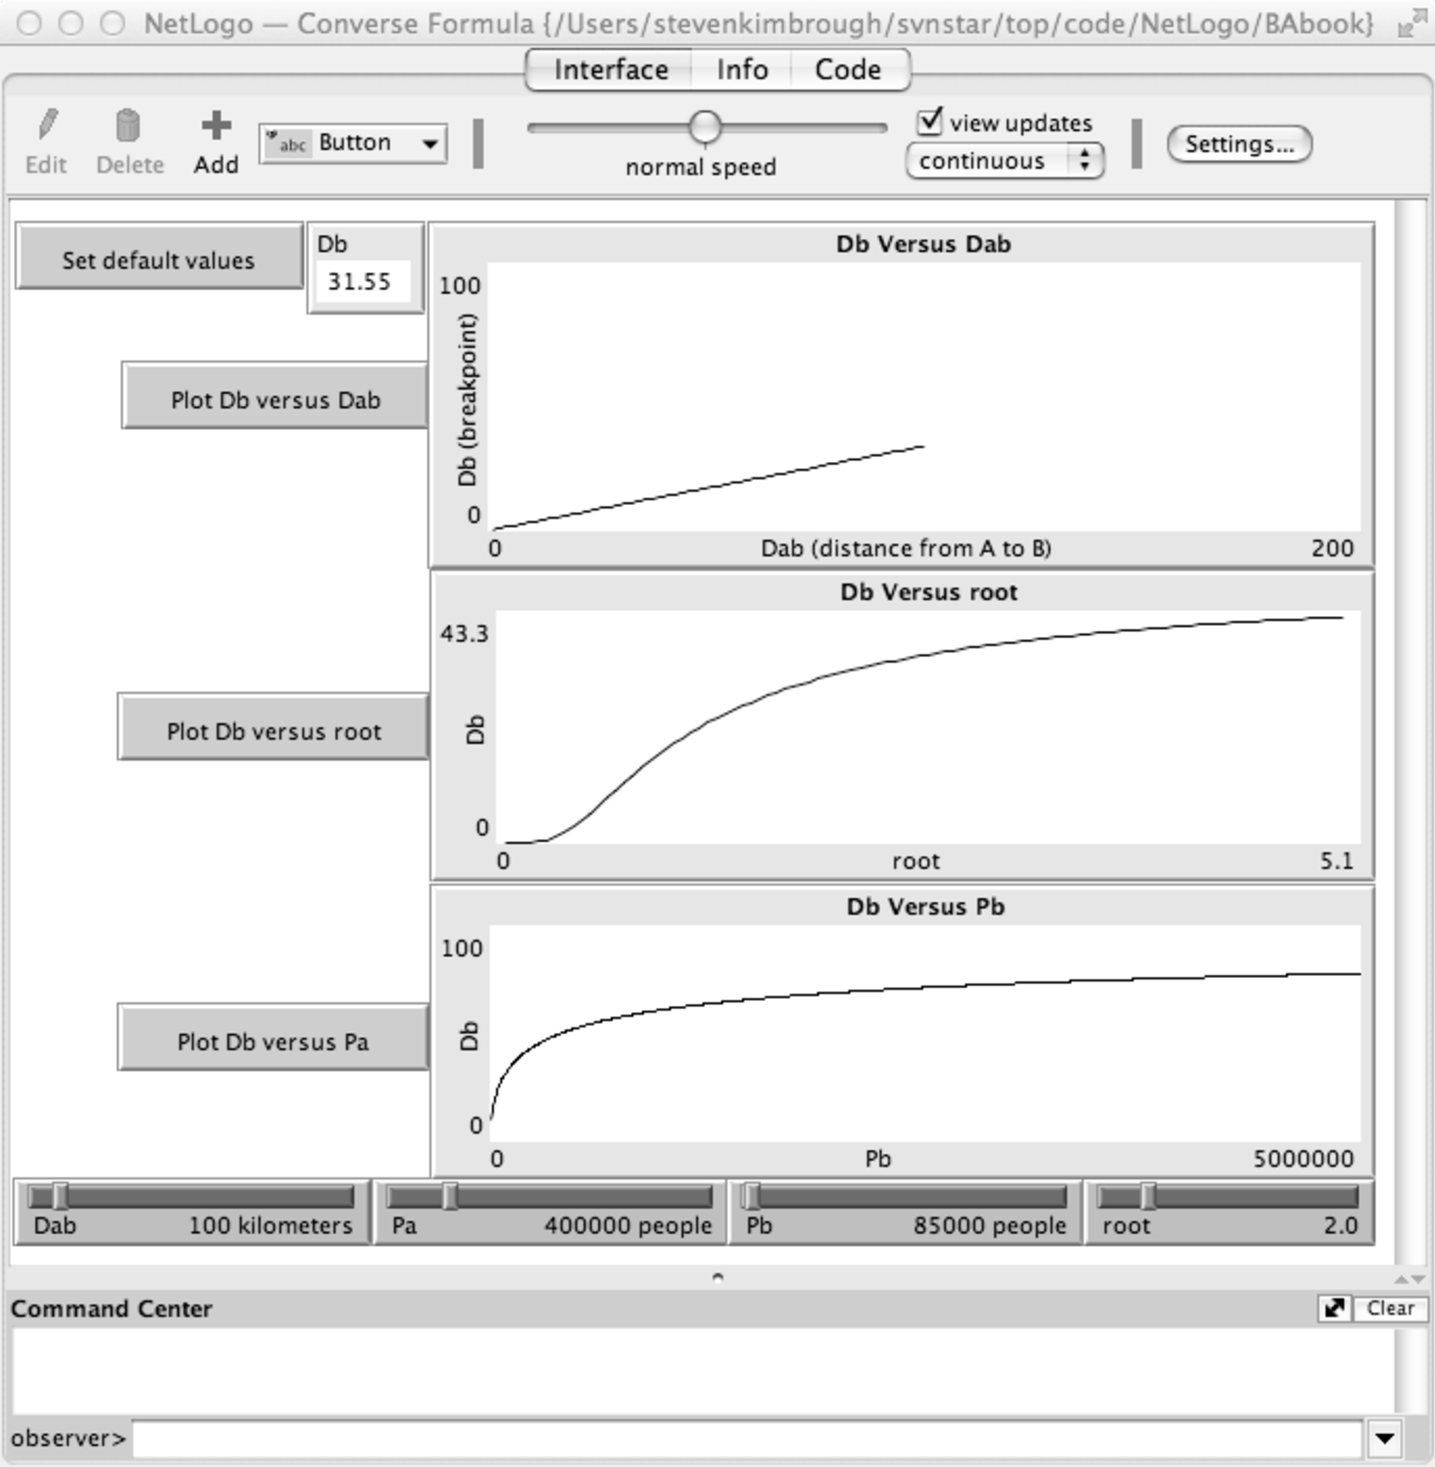
\includegraphics[width=\textwidth]{figures/ConverseFormula1.pdf} 
   \caption{Converse Formula model, a NetLogo implementation of Converse's formula.}
   \label{fig:converseformulanlogo}
\end{figure}

The four parameters of the model may be set by adjustable sliders at the bottom of the interface window: $D_{ab} \Rightarrow$ {\tt Dab}, $P_a \Rightarrow$  {\tt Pa}, $P_b \Rightarrow$ {\tt Pb}, and $r \Rightarrow$ {\tt root}. As you move them, the value of $D_b$ ($\Rightarrow$ {\tt Db}) is recalculated at displayed in a small labeled box (a NetLogo \emph{monitor}) at the top of the window. In Figure \ref{fig:converseformulanlogo} its value is 31.55. If you right-click on this monitor a new window will pop up displaying the implementation of the formula. Figure \ref{fig:converseformulaexpressionnlogo} shows what you will see.

The three plots in Figure \ref{fig:converseformulanlogo} let us chart how $D_b$ responds to changes in $D_{ab}$, {\it root}, and $P_b$ respectively, taken one at a time.


\begin{figure}[htbp] %  figure placement: here, top, bottom, or page
   \centering
   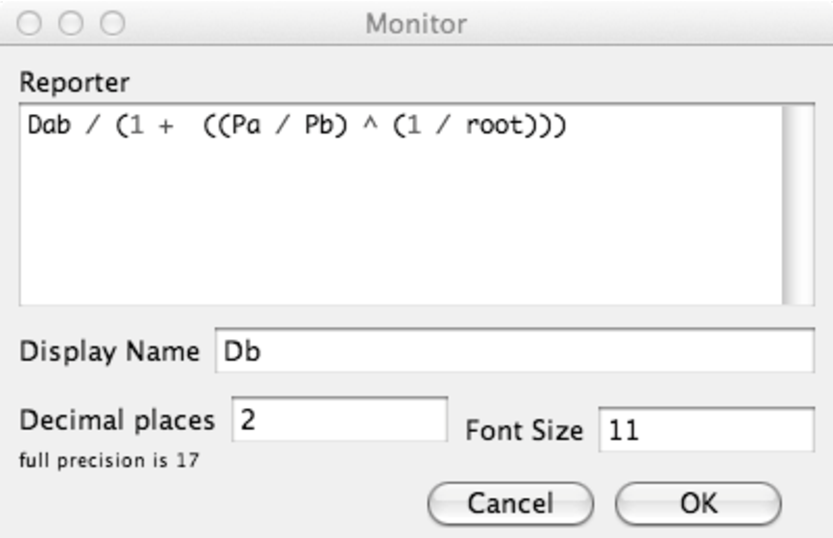
\includegraphics[width=\textwidth]{figures/ConverseFormulaFormula.pdf} 
   \caption{NetLogo implementation of the Converse formula expression, in a monitor widget.}
   \label{fig:converseformulaexpressionnlogo}
\end{figure}

\subsection{Employment of the Model\label{sec:converse_employment}}


The Converse formula tells us that if cities $A$ and $B$ are 100 kilometers apart,  city $A$ has a population of 400,000, and city $B$ has a population of 85,000, then the breakpoint is at about 31.55 kilometers. 

Besides implementing the Converse formula and letting us easily and quickly calculate it for different values of the parameters, the model supports us in exploring various \emph{post-solution analysis and exploration}\index{post-solution analysis} questions, such as:
\begin{enumerate}
\item How large would the population of city $B$ need to be in order for the breakpoint to be at least 37.0?
\item How small would the population of city $A$ need to be in order for the breakpoint to be at most 40.0?
\item Given fixed values of the other three parameters and a $D_b$ value that has a margin of safely of 5 kilometers for maintaining profitability, over what range of $r$ do we remain within this margin of safety?
\end{enumerate}


%\subsection{Points Arising}
%
%\begin{enumerate}
%\item The example is much simplified for the sake of illustrating the computational problem solving cycle.
%\item The example is nonetheless realistic. With various elaborations, businesses have used Converse's formula for exactly the purpose shown.
%\item That said, the \emph{Huff model} embodies a more sophisticated, generally better approach and is very widely used \cite[page 433]{eiselt_marianov_eds_2011}. 
%
%We should ask ourselves what the possible problems or limitations are of Converse's formula. Asking these and related questions is always an important aspect of analytics and thinking with models. Criticizing---thinking critically about---models and other representations is a necessary part of using them well.
%
%\item Learning about the elaborations that can be done in general---with other kinds of models and other kinds of problems---will be a prime item of focus as we move forward.
%\end{enumerate}

\clearpage

\section{Scoping Out Post-Solution Analysis}

Because post-solution analysis figures so importantly in what follows we shall discuss it now in some detail, describing the several facets of the concept. Later chapters will refer to this section and elaborate upon it.

\subsection{Sensitivity}

To begin, it is very often not a good assumption that each of the model's parameters---$D_{ab}$, $P_a$, and $P_b$ in the case of Converse's formula---are known with a very high degree of certainty. We can estimate them, with more or less precision, and solve the model on the basis of our best estimates, but when it comes to implementation of any decision, we may find that our best estimates in fact vary from reality. This is most often the case, and 
if so, then a number of \emph{sensitivity analysis} questions arise, prototypically:

\begin{quote}
{\it Are there small changes in parameter values that will result in large changes in outcomes according to the model?  If so, what are they and which parameters have the largest sensitivities, i.e., which parameters if changed by small amounts result in large changes in model outcomes? Which parameters have small sensitivities?}
\end{quote}
Points arising:
\begin{enumerate}
\item What counts as a large change or a small change to a parameter depends, of course, entirely on the context and the ambient levels of uncertainty.  Typically, we might think of changes on the order of a few percent in the level of a parameter as small. Perhaps a better measure is the amount of uncertainty or of variation not subject to our control in the value of a parameter. In the present case, perhaps $P_a$ is only comfortably certain within, say, 5\%\ of its assumed value. If so, we have a natural range of exploration for sensitivity analysis.

%In the present case, if the costs of the grains, the $c_j$'s, vary unpredictably $\pm$\$8 from the stated values, then that is a natural range to use for sensitivity analysis.
\item What counts as a large change or a small change in the outcome(s) of the model depends in large part on the model in question and on the overall context. In an application of the Converse formula we might had a policy constraint to the effect that, say, $D_b$ must be greater than 31 if we are to build store $B$ in the presence of $A$. We will naturally be interested in whether the results of the model are feasible in this sense and, with sensitivity analysis, whether small changes in the parameter values will make feasible (constraint satisfying) results infeasible (constraint violating) and vice versa. This will especially be the case with optimization models
 (our discussion of these begins in chapter \ref{COM_intro}), where we will be interested in knowing whether any small change in parameter values will make the model infeasible.  That is, if we make some ``small'' changes (however defined) to the model's parameters and then re-solve the model, could we find that there are no longer \emph{any} feasible solutions?
\item Less drastically, while we might be confident that small changes in the realized parameter values will not lead to infeasibility, there remains the possibility that small changes can drastically degrade the value of the optimal solution based on the estimated parameter values. In the present case, is it possible or likely that a small change to $P_a$ or $P_b$ would greatly change the value of our  present solution?   Could it happen, we must ask, that the present results  to the model would have disastrous consequences if implemented in the presence of very minor parameter value changes?
\item We are also interested in knowing which parameters are comparatively insensitive, so that relatively small changes to them have very little effect on outcomes upon implementing the  solution to the model.
\item We will need to consider all of our sensitivity questions both in the context of changes to a single parameter and to the context of simultaneous changes to multiple parameters.
\end{enumerate}
These are among the main general considerations for sensitivity analysis. The literature is extensive and the topic itself open-ended. These remarks  indicate the spirit of sensitivity analysis as a means of opening, rather than closing, the discussion of its scope and extent.

\subsection{Policy}

In a second category of post-solution analysis questions, the possibility may arise of altering decision variable levels because of considerations not reflected in the model. This possibility is  often present, and 
if so, then a number of \emph{policy analysis} questions arise, prototypically:

\begin{quote}
{\it Are there policy reasons, not represented in the model, for deviating  from either choosing a preferred (e.g., optimal) solution identified by the model or for modifying one or more parameter value? If so, what changes are indicated and what are the consequences of making them? Policy questions are about factoring into our decision making qualitative factors or aspects of the situation that are not represented in the model formulation.
}
\end{quote}
In a typical case, it may be desired for business reasons to set a decision variable to at least a minimal level. To take ta hypothetical example, there may be reasons having to do with, say, maintaining supplier relationships, for purchasing at least 70 units of grain 2, instead of the 50 that is optimal in terms of the model. The analysis question is then how best to do this and figuring out how much it will cost. If costs are too high that may well override any policy factors. In this typical mode of decision making, policy issues may be ignored and the model solved, after which an investigation in undertaken to determine whether to make changes in accordance with the policy factors.

What we are calling policy questions  frequently raised as what are referred to as \emph{intangibles,} factors that matter but are difficult to quantity, difficult certainly to express adequately  as part of a mathematical programming (or other model) formulation.  The model, however, can be most helpful for deliberations of this kind. If, to continue the example, there are policy reasons for favoring purchase of at least 70 units of grain 2, then the model can be used to estimate our opportunity cost were we to do this. Generally speaking, having a solution to the model at hand is materially useful for evaluating the cost of taking a different decision. Which decision to take is always up to the decision maker. A model serves its purpose well when it informs the decision maker about the costs and benefits of alternatives.\footnote{Thanks to Frederic H. Murphy for emphasizing to us the vital importance for model-based decision making of qualitative, extra-model factors, which we call \emph{policy questions.}}

\subsection{Outcome Reach\label{psa:outcome_reach}}

\index{outcome reach}
In the present example, the model outcome is $D_b$ = 31.55. What if instead of 31 we require at least 33? What combinations of parameter value changes will achieve this? and among them, how likely are they to be realized or achievable with action on the part of the decision maker?

%At optimality the objective function of our objective function has the value 19,550. That we are maximizing implies we would prefer to have a larger value. What would it take, what changes would have to be made to the model parameters, if we are to improve the objective function value to, say, 20,000? 

This is an example of an \emph{outcome reach} question on the improvement side. There are degradation side questions as well. For example, anything less than 29 might be disastrous. What combinations of parameter changes would lead to such a result, how likely are they, and what might we do to influence them?
%For example, we might it acceptable to have an objective value of at least 19,000. Were we to accept a degraded (here, reduced) objective value, what useful resources could be freed up for other purposes? 
Prototypically for this third category of post-solution analysis questions we have:

\begin{quote}
{\it Given an outcome predicted or prescribed by the model, and a specific desired alternative outcome, how do the assumptions of the model need to be changed in order to reach the desired outcome(s)? Is it feasible to reach the outcome(s) desired? If so, what is the cheapest or most effective way to do this? Outcome reach questions arise on the degradation side as well. By opting to accept a degraded outcome we may free up resources that can be used elsewhere.}
\end{quote}

\subsection{Opportunity}

Looking forward to constrained optimization models (chapter \ref{COM_intro} and later),  consider properties of a model discussed in chapter \ref{LP_intro}.
At optimality the constraints on nutrients A and B are \emph{tight.} In our model formulation, Figure \ref{fig:Wagner_Diet_model}, expression (\ref{wagner_diet_A_constraint}) states the constraint that the mix of feeds must provide at least 1,250 units of nutrient A, and expression  (\ref{wagner_diet_B_constraint}) states the constraint that the mix of feeds must provide at least 250 units of nutrient B. As we shall see, in the optimal solution both of these constraints are satisfied with equality. That is, in the optimal solution we supply exactly 1,250 units of nutrient A and 250 units of nutrient B. This raises the possibility that for a price we might be able to relax one or more of these constraints and thereby get a better result. %Relaxing a $\ge$ constraint means decreasing its right hand side parameter value (its $b_i$); conversely we relax a $\le$ constraint by increasing its right hand side value.

Prototypically, and more generally, for this fourth category of post-solution analysis questions we have:
\begin{quote}
{\it What favorable opportunities are there to take action resulting in changes to the assumptions (e.g., parameter values) of the model leading to improved outcomes (net of costs and benefits)?}
\end{quote}
These have also been called \emph{candle lighting questions} in allusion to the motto of the Christopher Society, ``It is better to light one candle than to curse the darkness'' \cite{kimbrough-et-al-june-1992,kimbrough-oliver-pritchett_1993,kimbrough-oliver-wits_1992,kimbrough-oliver-hicss_1994,kimbrough_wood_CIST_2008}.\index{candle lighting questions}
\label{first:candle_lighting}


\subsection{Robustness}

Something is robust if it performs well under varying conditions \cite{kimbrough_kuo_lau_2011_MIC}. Wagner's characterization is representative and applies to any system: ``A biological system is robust if it continues to function in the face of perturbations''  \cite[page 1]{wagner_andreas_2005}, although  we will normally want to add ``well'' after ``function''. (See also \cite{felix_wagner_2008,kirschner_gerhart_1998}.) This general notion of robustness is apt for, is important for, and is useful in many fields, including biology, engineering, and  management science.  The general notion, however, must be operationalized for specific applications. We focus in this book on management science applications, especially applications to optimization. 

 This fifth category of post-solution analysis questions may be summarized with:
\begin{quote}
{\it Which solutions or policy options of the model perform comparatively well across the full range of ambient uncertainty for the model? }
\end{quote}
How exactly we operationalize the general concept of robustness, in the context of decision making with models, requires extensive discussion which will appear in the sequel as we discuss various examples.

\subsection{Explanation}

Models, especially optimization models, are typically used \emph{prescriptively,} used that is to recommend courses of action. An optimal solution comes with an implicit recommendation that it be implemented. Because it is optimal the burden of proof for what to do shifts to any envisioned alternatives. In fact much of what post-solution analysis is about is deliberating whether to take a course of action other than that given by the optimal solution at hand.

It is natural in this context for any decision maker to request an explanation of \emph{why} what is recommended is recommended.  Why $X$ rather than some favored alternative $Y$?

\begin{quote}
{\it Why $X$?: Given a predicted or prescribed outcome of the model, $X$, why does the model favor it?  Why not $Y$?: Given a possible outcome of the model, $Y$, why does the model not favor it it over $X$?}
\end{quote}
Questions of this sort are quite often encountered in practice and handed with appeal to common sense.  For example, constraints might be added to the model to force the outcome $Y$. This will result either in a degraded objective function value or outright infeasibility. In either case, the model can be helpful in explaining why $Y$ is inferior to to $X$, particularly by suggesting outcome reach analyses that add insight (e.g., that the price on a certain parameter would have to fall by at least a certain amount).

Although explanation questions are commonly engaged it remains true that their is neither settled doctrine or methodology on how best to undertake explanatory analysis with optimization models, nor is there bespoke software support for it. Practice remains unsystematic in this regard.
The pioneering work by Harvey Greenberg in the context of linear programming---
\cite{greenberg_1993_JulyAugust,greenberg_1993_SeptOct,greenberg_1993_NovDec,greenberg_1994_JanFeb}---remains the point of contemporary departure.

\subsection{Resilience}

Robustness and resilience are closely related concepts. Neither is precisely defined in ordinary language. More careful usage requires a degree of stipulation---``This is what we shall mean by\ldots ''---and many such stipulations have been given, if only implicitly. In short, the terms do not have established standard meanings, and the meanings that have been given are various and mutually at odds. We shall use robustness as described above: something is robust if it works reasonably well under varying conditions. We reserve resilience for a form of robustness achieved by action in response to change. A robust defense resists attack by being strong in many ways, in the face of multiple kinds of aggressive forays. A resilient defense is robust in virtue of an effective response to an attack. 

Robustness may be static or dynamic. Resilience is dynamic robustness. A resilient solution is one that affords effective decision making after now-unknown events occur. While it is generally desirable to delay a decision until more information is available, this might not be possible or it may come with a prohibitive cost. In some cases, clever design will permit delayed decision making or put the decision maker in position to adapt cheaply to a number of possible eventualities.

% real options. stochastic programming and recourse. expected value of sample information in decision analysis

Summarizing, these are prototypical resilience (dynamic robustness) questions.
\begin{quote}
{\it Which decisions associated with the model are the most dynamically robust? That is, which decisions best afford deferral of decision to the future when more is known and better decisions can be made?}
\end{quote}

\centerline{* * *}

Figure \ref{fig:post_solution_questions}, page \pageref{fig:post_solution_questions}, summarizes
our seven categories of post-solution analysis questions. We emphasize that boundaries are fuzzy and urge the reader to attend less to clarifying the boundaries and more to using the framework to suggest useful questions leading to better decisions. We mean our framework to stimulate creative deliberation, rather than to encode settled knowledge. Decision making with any model occurs within a context broader than the model. That context may be simple and straightforward, it may be complex and heavily strategic, involving consideration of possible actions by many other decision makers, and it may be anywhere in between.

% Fred's point about game versus non-game contexts.






%/* 1. Plus decision variable levels. Perhaps a minimum level of certain grains is necessary or valuable. */
%
%/* 2. candle-lighting \cite{kimbrough-et-al-june-1992,kimbrough-oliver-wits_1992,kimbrough-oliver-pritchett_1993,kimbrough-oliver-hicss_1994}
%
%/* 3. structural versus parametric post-solution analysis */
%
%/* 4. Harvey G. explanation */
%
%In short, during post-solution analysis we may want to consider:
%\begin{enumerate}
%\item Parameter uncertainties
%\item Policy-based decision variable setting (away from optimality in the model)
%\item Candle-lighting analysis
%\item 
%\end{enumerate}


\begin{figure}[h]
\figtop
\begin{enumerate}
\item Sensitivity

Are there small changes in parameter values that will result in large changes in outcomes according to the model?  If so, what are they and which parameters have the largest sensitivities, i.e., which parameters if changed by small amounts result in large changes in model outcomes? Which parameters have small sensitivities?

\item Policy


Are there policy reasons, not represented in the model, for deviating  from either choosing a preferred (e.g., optimal) solution identified by the model or for modifying one or more parameter value? If so, what changes are indicated and what are the consequences of making them? Policy questions are about factoring into our decision making qualitative factors or aspects of the situation that are not represented in the model formulation.


\item Outcome reach

Given an outcome predicted or prescribed by the model, and a specific desired alternative outcome, how do the assumptions of the model need to be changed in order to reach the desired outcome(s)? Is it feasible to reach the outcome(s) desired? If so, what is the cheapest or most effective way to do this? Outcome reach questions arise on the degradation side as well. By opting to accept a degraded outcome we may free up resources that can be used elsewhere.

\item Opportunity

What favorable opportunities are there to take action resulting in changes to the assumptions (e.g., parameter values) of the model leading to improved outcomes (net of costs and benefits)?

\item Robustness

Which solutions or policy options of the model perform comparatively well across the full range of ambient uncertainty for the model? %Which decisions associated with the model will 

\item Explanation

Why $X$?: Given a predicted or prescribed outcome of the model, $X$, why does the model favor it?  Why not $Y$?: Given a possible outcome of the model, $Y$, why does the model not favor it it over $X$?

\item  Resilience

Which decisions associated with the model are the most dynamically robust? That is which decisions best afford deferral of decision to the future when more is known and better decisions can be made?
\end{enumerate}
% 2014-11-22: Yesterday I showed this briefly to Fred Murphy, who wanted to add two items: 8. Weighing qualitative factors/aspects in choices and 9. individual versus group decision making (and concomitant strategic/gaming issues). I am folding 8 here into 2 (policy) and for now ignoring 9. Later, we can distinguish two modes, individual and group or social decision making. So, I think the list should remain as is with 7 items.
\caption{Seven categories of representative questions addressed during post-solution analysis.}
\label{fig:post_solution_questions}
\figbot
\end{figure}

\clearpage

\section{Parameter Sweeping: A method for post-solution analysis\label{sec:parameter_sweep_intro}}

\index{parameter sweeping}

Briefly put, a parameter sweep of a model is an experiment in which multiple model outcomes are produced by executing an algorithm numerous times that solves the model with different parameter configurations.
NetLogo, with its BehaviorSpace feature,  emphasizes parameter sweeping as a key part of modeling.  This is  from the {\it NetLogo User Manual}\,:\index{BehaviorSpace}
\begin{quote}
BehaviorSpace is a software tool integrated with NetLogo that allows you to perform experiments with models.

BehaviorSpace runs a model many times, systematically varying the model's settings and recording the results of each model run. This process is sometimes called ``parameter sweeping''. It lets you explore the model's ``space'' of possible behaviors and determine which combinations of settings cause the behaviors of interest.
\end{quote}

\noindent Of course we can do parameter sweeping without recourse to NetLogo. To illustrate, the following code implements the Converse formula in \mlb . 

\begin{quote}
\begin{verbatim}
function [ Db ] = converse_formula( Dab, Pa, Pb )
%converse_formula Calculates the Converse formula.
% Dab is the distance between establishment a and
% b. Pa is the population of a, Pb is the population
% of b. Db = Dab/(1 + sqrt(Pa/Pb)). Db is the
% predicted distance from b in the direction of a
% before which customers will go to b, after which
% customers will go to a.
Db = Dab / (1 + sqrt(Pa/Pb));
end
\end{verbatim}
\end{quote}
It is not necessary for present purposes that you understand this code, although we imagine that its meaning is reasonably clear. The important point is that once a model is implemented and executable on a computer (as this \mlb\ function is) we can write a program that iteratively feeds it different parameter values and collects the outputs, which are the resulting values of the function.

Specifically, we can set $P_a$ to a sequence of values, say 390,000, 395,000, 400,00 (our original value), 405,000, and 410,000, and we can set $P_b$ to a different sequence of values, say 75,000, 80,000, 85,000 (our original value), 90,000, and 95,000. This yields $5\times 5 = 25$ distinct parameter combinations for which we can obtain function values by executing the Converse function code.
Table \ref{table:converse_parameter_sweep} presents the results of calculating the Converse formula for these 25 combinations of parameter values.

\begin{table}[t]
\figtop
\begin{center}
\begin{tabular}{r|rrrrr}
   & 75000 & 80000 & 85000 & 90000 & 95000 \\ \hline
 390000 & 30.4845 & 31.1727 & 31.8267 & 32.45 & 33.0453 \\ 
395000 & 30.3497 & 31.0362 & 31.6887 & 32.3105 & 32.9046 \\ 
400000 & 30.2169 & 30.9017 & 31.5527 & 32.1731 & 32.7659 \\ 
405000 & 30.0861 & 30.7692 & 31.4187 & 32.0377 & 32.6292 \\ 
410000 & 29.9572 & 30.6387 & 31.2866 & 31.9043 & 32.4945 \\ 
\end{tabular}
\end{center}
\caption{Parameter sweep results for the Converse formula. Rows: $P_a$ values. Columns: $P_b$ values.}
\label{table:converse_parameter_sweep}
\figbot
\end{table}

This simple example may serve as a prototype for much that is to come. We will confine ourselves here to just two points.
\begin{enumerate}
\item In two dimensions, by sweeping two parameters as in Table \ref{table:converse_parameter_sweep}, it becomes natural to think of the ensemble on a geographic analogy. We see in the present case that when $P_b$ is equal to or greater than 85,000, the formula value exceeds 31, regardless of the $P_a$ values present. More precisely, when $P_b \ge$ 85,000 or when $P_b$ = 80,000 and $P_a \le 395,000$, the function value exceeds 31; otherwise it does not. Thus, with our constraint of 31, discussed above, we see two regions or two \emph{phases} of the parameter space revealed by the sweep.

This point, that parameter sweeping may reveal regions or phases of interest applies, of course, to ensembles of more than two parameters. And it applies to models of all kinds.

\item Generalizing further, parameter sweeping \emph{when it is practicable} can be used as a basis for answering all or nearly all of our post-solution analysis questions. This is a subject we will develop in depth throughout the book.
\end{enumerate}

\section{Discussion}

We have introduced the computational problem solving cycle and Converse's formula as a very simple example of it, along with an implementation of the formula as a NetLogo model, {\it Converse Formula.nlogo.}

We chose the Converse formula example  for the sake of illustrating the computational problem solving cycle.
The example is nonetheless realistic.  Businesses have used Converse's formula, with various elaborations, for exactly the purpose shown.

A point of emphasis here and throughout the book is that analytics are not static. To do business analytics we need to exercise implementations in order to  explore our models and data.  Obtaining a solution---a number from a model, a plot of a body of data, and so on---is hardly enough. Business analytics is above all about \emph{post-solution analysis and exploration.}\index{post-solution analysis}
For this purpose, implementations  should be seen as providing tools for exploration. The convenient graphical user interface  supplied by the Converse Formula NetLogo should be seen as an elementary example of an \emph{analytics dashboard}.\index{dashboard!analytics}\index{analytics dashboard} These concepts will be with us throughout as we delve into business analytics.



\section{For Exploration}

\begin{enumerate}
\item Critically assess the Converse formula as a model. What are its strengths? limitations? key assumptions? Under what conditions is it likely to be useful? not very useful?
\item In addition to the post-solution analysis questions discussed in \S\ref{sec:converse_employment} for the Converse formula, what other interesting questions are supported by the Converse Formula NetLogo model? Discuss and explain why they are interesting or likely to be useful. What about interesting questions that are not well supported by the model?
%\item As presented, the Huff model seems to assume that every person will shop at one store or another. Surely this is an unrealistic assumption. Comment and discuss. Does it invalidate the model? How might the model be used in a valid fashion?  How might the model be revised to make it more valid?
%\item \ldots [especially, sensitivity analysis questions, plotting]
\item The following passage appears at the end of \S\ref{sec:computational_problem_cycle}.
\begin{quote}
\ldots we might frame [Figure \ref{fig:computational_problem_solving}] as an updating or complement for the twenty-first century and new technology of Peirce's ``The Fixation of Belief''  \cite{peirce_fixation}. 
\end{quote}
Really? Do you agree? or not? Discuss.
\item What is the epistemological status of Converse's formula? It is evidently not a law of nature, although it is expressed like one. Does it support counterfactuals? Is it true?
\item Reimplement the Converse Formula NetLogo model in a spreadsheet program, such as Excel. Compare and contrast the two implementation environments, NetLogo and spreadsheets, for this purpose.
\item Reimplement the Converse Formula  NetLogo model in Python. Compare and contrast the two implementation environments, NetLogo and Python, for this purpose.

\item Assuming we have a model for which extensive parameter sweeping results can be obtained. Discuss how to use parameter sweeping to answer the questions of post-solution analysis, discussed in the chapter.
\end{enumerate}



